%\documentclass[tikz]{beamer}
\documentclass[notheorems]{beamer}

%\usepackage{tikz}
%\usetikzlibrary{shapes,arrows}
\mode<presentation>{}
\usepackage{beamerthemeshadow}
%\let\definition\relax
\let\theorem\relax
\input{../../paperProduction/occBind/docs/AMArepresentationNewCmds}


\author{Gary S. Anderson\thanks{The analysis and conclusions set forth are those of the author and do not indicate concurrence by other members of the research staff or the Board of Governors.}}

\title{A New Series Representation for 
Nonlinear Dynamic Stochastic Model Solutions: General Error Bounds and a New Solution Algorithm}

\date{\today: \currenttime}
\begin{document}


\begin{frame}
\maketitle
\end{frame}

\section{Introduction and Summary}

\begin{frame}
  \frametitle{Outline}
  \begin{itemize}
  \item Introduction
  \item Summary of Results
  \item The Series Representation
  \item Model Error Bounds
  \item A New Solution Algorithm
  \end{itemize}
\end{frame}

\subsection{Introduction}
\label{sec:introduction}


\begin{frame}
  \frametitle{Introduction}
\begin{itemize}
\item Model solutions characterized by :

\begin{gather}
\eqnFuncSys \intertext{ where, each }
\eqnFuncSysI{i}\equiv \eqnFuncSysIExpl{i} \label{eqnGates}
\end{gather}
\item Boolean valued gate, $\gate_i$. 
\item model equations, $\eqnFunc_i$,  
\item ``Auxiliary variables'' if necessary
\item exhaustive and mutually exclusive determining the solution  $x_t\tArg$
\end{itemize}
\end{frame}

\subsection{Summary of Results}
\label{sec:summary-results}




\begin{frame}
  \frametitle{Model Error Bounds}
  \begin{itemize}
  \item Exact (typically unknown) solution $x^\star_t=g^\star(x_{t-1},\epsilon_t)$ 
  \item Proposed solution  $x^p_t=g^p(x_{t-1},\epsilon_t), \,\,G^p(x)\equiv \expct{g^p(x_{t-1},\epsilon_t)}$ 
 \item Euler errors $\eulerE_i\tArg \equiv  \eqnFunc(x_{t-1},g^p(x_{t-1},\epsilon),G^p(g^p(x_{t-1},\epsilon)),\epsilon)$
 \item We can easily compute matrices  $F, \phi $ such that 
 {\small   \begin{gather*}
 \someNorm{ x^\star_{t}(x_{t-1},\epsilon) -	 x^p_{t}(x_{t-1},\epsilon)} \le 
 \max_{\{i,x_{t-1},\epsilon\}} \someNorm{(I-F)^{-1} \phi \eulerE_i\tArg }
    \end{gather*}}
  \end{itemize}
\end{frame}
\begin{frame}
  \frametitle{Alternative Error Bounds}
  \begin{itemize}
  \item \cite{judd2017lower}
  \item \cite{peralta-alva14}
  \item \cite{santos2005accuracy}
  \item \cite{Santos2000accuracy}
  \end{itemize}
\end{frame}




\begin{frame}
  \frametitle{A New Algorithm}
 {\small  
\begin{itemize}
\item Using a formula from \citep{anderson10},
 \item Any bounded time invariant discrete map can be written as
    \begin{gather*}
      	 x\tArg =B x_{t-1}+ \phi \psi_\epsilon\epsilon + (I - F)^{-1} \phi \psi_c + \sum_{\sForSum=0}^\infty F^\sForSum \phi \ZWOarg(\expct{x_{t+\nu}})\\ \intertext{ so that}
\expct{ x_{t+1}\tArg} =B x\tArg  + (I - F)^{-1} \phi \psi_c+ \sum_{\sForSum =1}^\infty F^{\sForSum-1} \phi \ZWOarg(\expct{x_{t+\nu}}) 
    \end{gather*}
   \item If these functions satisfy the model equations you have a solution
   \item If not, use the $\eulerE_i \text{ and } \eqnFuncSys $ information to improve the solution
  \end{itemize}
}
\end{frame}

\begin{frame}
  \frametitle{Alternative Approaches}
  \begin{itemize}
\item \cite{Judd2014}
\item \cite{juddGSSA2011}
\item \cite{holden15:_exist_dsge}
\item  \cite{guerrieri15:_occbin}
  \end{itemize}
\end{frame}

\begin{frame}
  \frametitle{Advantages of the Series Formulation}
  \begin{itemize}
  \item Builds upon existing approaches
    \begin{itemize}
    \item Uses the an-isotropic Smolyak Method and adaptive paralletope method
    \end{itemize}
  \item Precomputes integrals
  \item Polynomial interpolation highly parallelizable
  \item very general functional form
  \end{itemize}
\end{frame}





\section{A New Series Representation For  Bounded Time Series}
\label{sec:newseries}

\subsection{Linear Reference Models and a Formula for  ``Anticipated Shocks''}
\label{sec:linref}



\subsection{ An  ``Arbitrary'' Linear Model and  Bounded Time Series}
\label{sec:almostarbitrary}



\begin{frame}
  \frametitle{Linear Reference Model}

  \begin{itemize}
  \item linear homogeneous system with  unique stable solution,  

\begin{gather}
  	 H_{-1} x_{t-1} + H_0 x_t + H_1 x_{t+1}=0\label{hSystem}
\end{gather}
\item inhomogeneous solutions 
\begin{gather}
	 H_{-1} x_{t-1} + H_0 x_t + H_1 x_{t+1}=\psi_\epsilon \epsilon +\psi_{c}
\intertext{ can be computed as}
x_t=B x_{t-1} + \phi \psi_\epsilon \epsilon + (I - F)^{-1} \phi \psi_c
\intertext{where}
\phi= (H_0 +H_1 B)^{-1}  \text{ and } \,\,F=-\phi H_1 
\end{gather}

\item Define $\linMod \equiv \linModMats$.
  \end{itemize}

\end{frame}
\begin{frame}
  \frametitle{Fully Anticipated Shocks}
{\small
\begin{theorem}
Arbitrary but bounded path
 \begin{gather*}
   \xWOarg_t \in{R^L}\,\text{ with }\,\infNorm{\xWOarg_t}  \le \bar{\mathcal{X}}\,\,\,\,\,\forall t> 0 
\intertext{ define  $  z_{t} \equiv H_{-1} \xWOarg_{t-1} +  H_0 \xWOarg_{t} +  H_1 \xWOarg_{t+1}   $ then }
	  \xWOarg_{t} =B x_{t-1}+ \phi \psi_\epsilon\epsilon + (I - F)^{-1} \phi \psi_c + \sum_{\sForSum=0}^\infty F^s \phi z_{t+\sForSum} \\
	  \xWOarg_{t+k+1} =B \xWOarg_{t+k}  + (I - F)^{-1} \phi \psi_c+ \sum_{\sForSum =0}^\infty F^\sForSum \phi z_{t+k+\sForSum+1} \,\,\,\,\,\forall t,k \ge  0.
	 \end{gather*}
\end{theorem}
}
\end{frame}

\subsection{A Numerical Example}
\label{sec:numerical-exampley}


\begin{frame}

  \frametitle{A Numerical Example}


\begin{gather}
  \begin{bmatrix}
H_{-1}&H_{0}&H_{1} 
  \end{bmatrix}=
\vcenter{\hbox{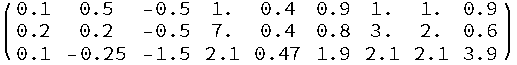
\includegraphics{refHmat.pdf}}}\intertext{with $\psi_c=\psi_\epsilon=0, \,\,  \psi_z=I$.}
  B=
\vcenter{\hbox{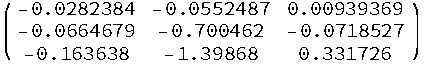
\includegraphics{refBmat.pdf}}}\\
\phi=
\vcenter{\hbox{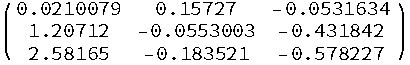
\includegraphics{refPhimat.pdf}}}\\
F=
\vcenter{\hbox{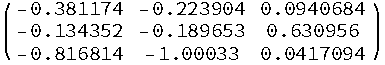
\includegraphics{refFmat.pdf}}}
\end{gather} 

  
\end{frame}

\begin{frame}
  \frametitle{Some Time Series}


\begin{figure}
  \centering
\begin{gather}
  x_{1,t}=\alpha D_\pi(t) \\
x_{2,t}=\beta (-1)^t\\
x_{3,t}=\epsilon_t 
\end{gather} 
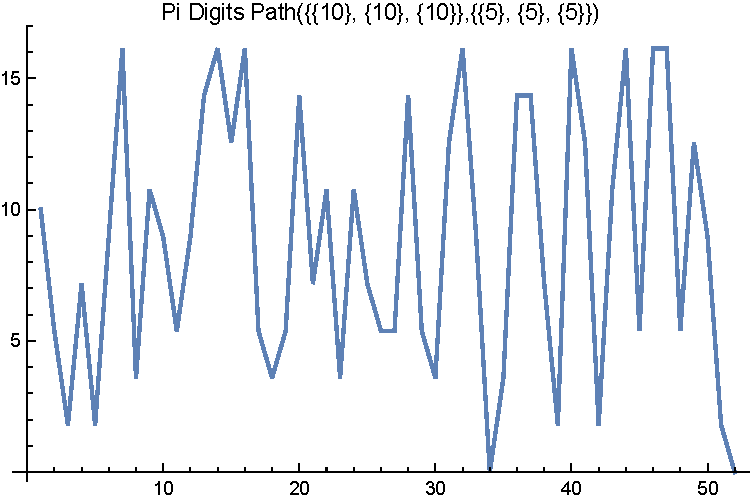
\includegraphics[width=1in]{piPath.pdf}
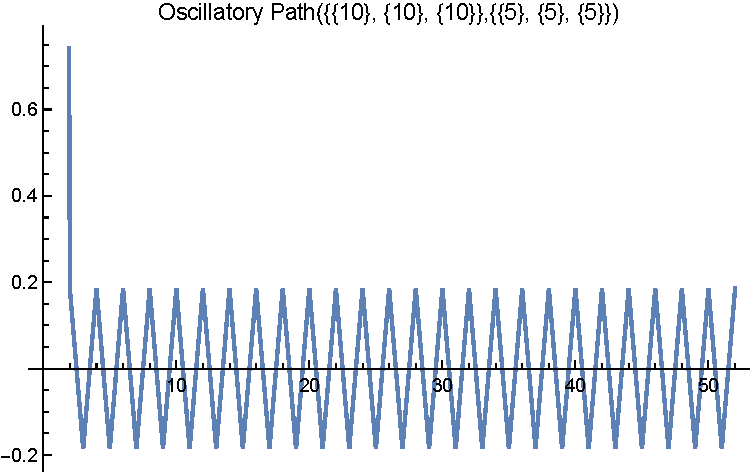
\includegraphics[width=1in]{oscillPath.pdf}
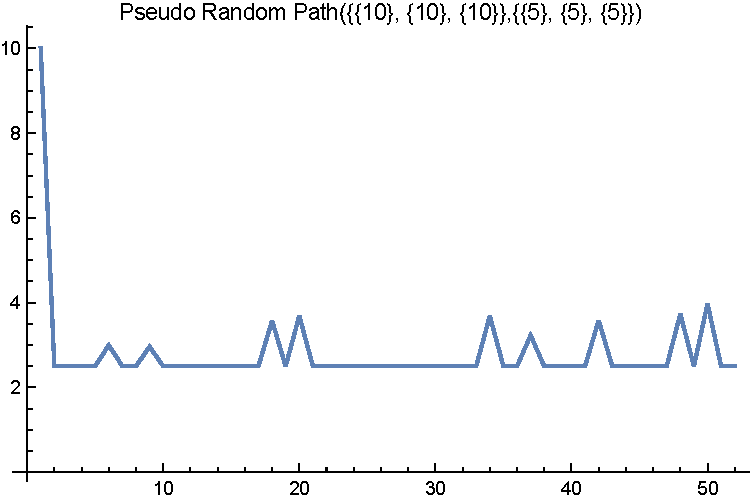
\includegraphics[width=1in]{pseudoPath.pdf}
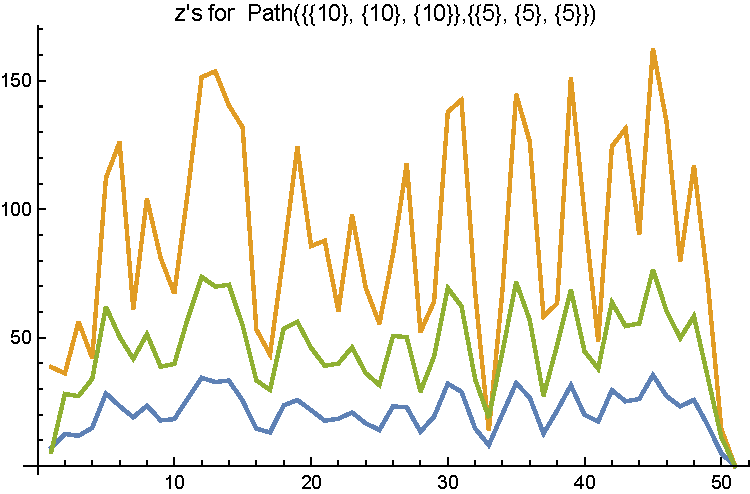
\includegraphics[width=1in]{theZs.pdf}  
  
  \caption{Arbitrary Bounded Time Series Paths and Corresponding $z_{i,t}$ values}\label{arbpaths}
\end{figure}



\end{frame}

\subsection{Assessing Errors}
\label{sec:assessing-errors}


\begin{frame}
  \frametitle{Truncation Error}
 	 \begin{gather}
 	 \xWOargK_t \equiv B x_{t-1}+ \phi \psi_\epsilon\epsilon  + (I - F)^{-1} \phi \psi_c + \sum_{s=0}^k F^s \phi z_{t}\label{theTruncSeries}
 \end{gather}
We can bound the  series approximation truncation errors.
Since
    \begin{gather}
      \label{eq:1}
\sum_{s=k+1}^{\infty} F^s \phi \psi_z = (I -F)^{-1} F^{k+1}\phi \psi_z       \\
\infNorm{\xWarg-\xWargK} \le\\ \infNorm{(I -F)^{-1} F^{k+1}\phi \psi_z} \left ( \infNorm{H_{-1} }+ \infNorm{H_{0} }+ \infNorm{H_{1} } \right )\bar{\mathcal{X}}
    \end{gather}

\end{frame}
\begin{frame}
  \frametitle{Truncation Error}


\begin{figure}
  \centering


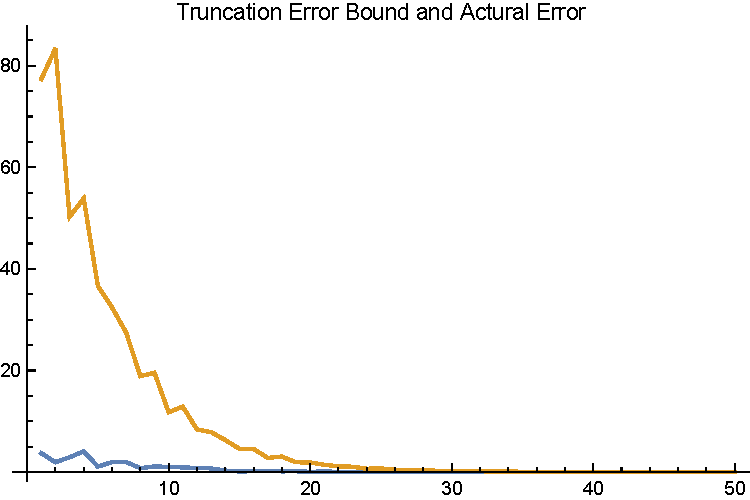
\includegraphics[width=3in]{arbTruncErr.pdf}  
  \caption{$x_t$ Error Bound Versus Actual Error} \label{figArbTrunc}

\end{figure}

\end{frame}

\begin{frame}
  \frametitle{Path Error}
One could consider approximating $\mathcal{X}_t$ using
 	 \begin{gather}
 	 \xWOargK_t \equiv B x_{t-1}+ \phi \psi_\epsilon\epsilon  + (I - F)^{-1} \phi \psi_c + \sum_{s=0}^\infty F^s \phi (z_{t}+\Delta z_{t})\label{theDeltaSeries}
 \end{gather}
We can bound the  series approximation  errors by using the largest $\Delta z_t$ in the formula. 

    \begin{gather}
\infNorm{\xWarg-\xWargK} \le \infNorm{(I -F)^{-1} \phi \psi_z}  \infNorm{\Delta z_t } \label{pathErr}
    \end{gather}

\end{frame}


\section{Nonlinear Dynamic Stochastic Time Invariant Maps}
\label{sec:extToMaps}



\subsection{Application to Time Invariant Maps}


\begin{frame}
  \frametitle{Time Invariant Maps}


  \begin{itemize}
\item  Many dynamic stochastic models 
  \begin{itemize}
  \item  have solutions that fall in this class.
\item  generate  bounded time series paths 
  \end{itemize}
  \end{itemize}



\subsection{An RBC Example}
\label{sec:rbcaux}
  We consider a model described in \cite{Maliar2005}\footnote{Here, we set their $\beta=1$ do not discuss quasi-geometric discounting or time-inconsistency.}
 \begin{gather*}
   \max\left \{  u(c_t) + E_t \sum_{t=0}^\infty  \delta^{t}u(c_{t+1})\right \}\\
c_t + k_t=(1-d)k_t + \theta_t f(k_t)\\
f(k_t)= k_t^\alpha\\
u(c)=\frac{c^{1-\eta}-1}{1-\eta}
 \end{gather*}
 \end{frame}

 \begin{frame}
   \frametitle{First Order Conditions}


The well known first order conditions for the model are

\begin{tcolorbox}[ams gather]
\frac{1}{c_t^{\eta}}=\alpha \delta k_{t}^{\alpha-1} E_t \left (\frac{\theta_{t}}{c_{t+1}^\eta} \right ) \\
c_t + k_t=\theta_{t-1}k_{t-1}^\alpha \\
 \theta_t =\theta_{t-1}^\rho e^{\epsilon_t}\label{rbcSys}
 \end{tcolorbox}

\label{sec:rbcexample}

When $\eta=d=1$, we have
{\small
 \begin{gather*}
   \begin{split}
\frac{1}{c_t}=\alpha \delta k_{t}^{\alpha-1} E_t \left (\frac{\theta_{t}}{c_{t+1}} \right ) \\
c_t + k_t=\theta_{t-1}k_{t-1}^\alpha \\
\theta_t =\theta_{t-1}^\rho e^{\epsilon_t}   \end{split} \text{   leading to a closed form solution}
\begin{split}
c_t=  (1-\alpha \delta) \theta_{t} k_{t-1}^\alpha\\
  k_{t}= \alpha \delta \theta_{t} k_{t-1}^\alpha.\label{soln}\\
\theta_t =\theta_{t-1}^\rho e^{\epsilon_t}.\end{split}
\end{gather*}
}
\end{frame}

\begin{frame}

  \begin{itemize}
  \item Mean zero iid $\epsilon_t$ 
  \item compute the conditional expectation of the model variables for any given $\theta_{t-1},k_{t-1}$
\begin{gather*}
  E_t(c_t|\theta_{t-1},k_{t-1})=(1-\alpha\delta)k_{t-1}^\alpha e^{\frac{\sigma^2}{2}}\theta_{t-1}^\rho\\
  E_t(k_t|\theta_{t-1},k_{t-1})=\alpha\delta k_{t-1}^\alpha e^{\frac{\sigma^2}{2}}\theta_{t-1}^\rho\\
  E_t(\theta_t|\theta_{t-1},k_{t-1})=e^{\frac{\sigma^2}{2}}\theta_{t-1}^\rho
\end{gather*}


\item applying the law of iterated expectations
\item   compute conditional expected solution paths forward from any initial values $(x_{t-1},\epsilon_t)$.
\item obtain series representation from the family of conditional expectations
along with the $\linMod$
  \end{itemize}

\end{frame}

\begin{frame}
  
{\small

For any given values of $k_{t-1},\theta_{t-1}, \epsilon_t$ the model solution and conditional expectations path produces paths for $z_{1t}\tArg, z_{2t}\tArg, z_{3t}\tArg$

\begin{gather*}
  \begin{bmatrix}
c_t(k_{t-1},\theta_{t-1}, \epsilon_t)\\
k_t(k_{t-1},\theta_{t-1}, \epsilon_t)\\
\theta_t(k_{t-1},\theta_{t-1}, \epsilon_t)
  \end{bmatrix} \rightarrow
  \begin{bmatrix}
  z_{1t}(k_{t-1},\theta_{t-1}, \epsilon_t)\\
  z_{2t}(k_{t-1},\theta_{t-1}, \epsilon_t)\\
  z_{3t}(k_{t-1},\theta_{t-1}, \epsilon_t) 
  \end{bmatrix}\equiv z(k_{t-1},\theta_{t-1}, \epsilon_t)\intertext{where}
  \begin{bmatrix}
c_t(k_{t-1},\theta_{t-1}, \epsilon_t)\\
k_t(k_{t-1},\theta_{t-1}, \epsilon_t)\\
\theta_t(k_{t-1},\theta_{t-1}, \epsilon_t)
  \end{bmatrix}  =
B   \begin{bmatrix}
c_{t-1}\\
k_{t-1}\\
\theta_{t-1}
  \end{bmatrix}  + \phi \psi_\epsilon\epsilon_t + (I - F)^{-1} \phi \psi_c +\\ \sum_{\sForSum=0}^\infty F^s \phi z_{t+\sForSum}(k_{t-1},\theta_{t-1}, \epsilon_t) 
\end{gather*}
}
\end{frame}
\begin{frame}
  



For example, using the following parameter values and using the arbitrary linear reference model we can generate a series representation for the model solutions.

\begin{gather}\label{rbcparams}
\vcenter{\hbox{\includegraphics{../../paperProduction/occBind/docs/RBCParamSubs.pdf}}} \,\, \text{ we have } \,\,
  \begin{bmatrix}
    c_{ss}\\k_{ss} \\ \theta_{ss} 
  \end{bmatrix}=
\left [ \vcenter{\hbox{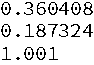
\includegraphics{RBCSSVal.pdf}}}\right ]
\end{gather}

With 
\begin{gather}\label{theInits}
  \begin{bmatrix}
 k_{t-1}\\\theta_{t-1}\\\epsilon_t 
  \end{bmatrix}=
\left [ \vcenter{\hbox{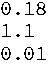
\includegraphics{anXEps.pdf}}}\right ]
\end{gather}

\end{frame}
\begin{frame}
  

\begin{figure}
  \centering
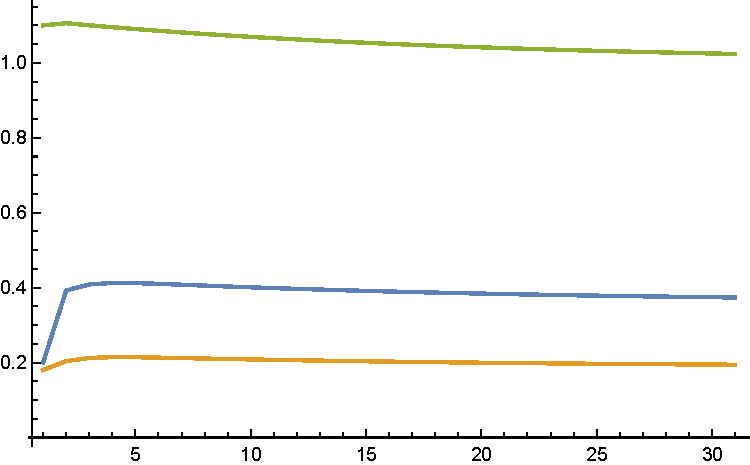
\includegraphics[width=1.7in]{simprbcvals.pdf}  
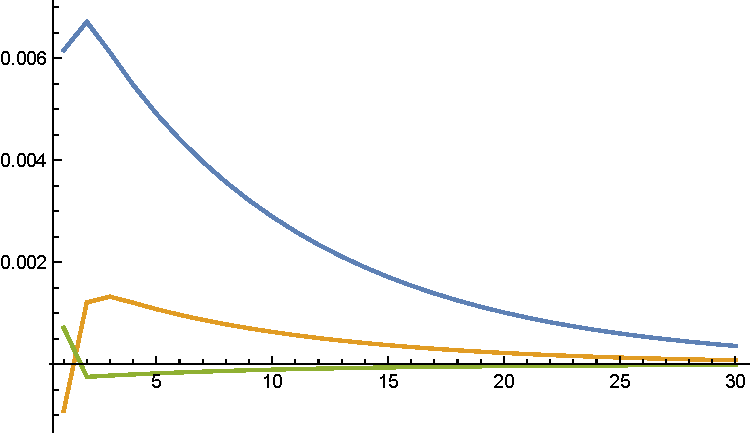
\includegraphics[width=1.7in]{simprbczvals.pdf}  
  \caption{model variable values and z values}
  \label{rbcpaths}
\end{figure}

\end{frame}

\begin{frame}
  

\begin{figure}
  \centering
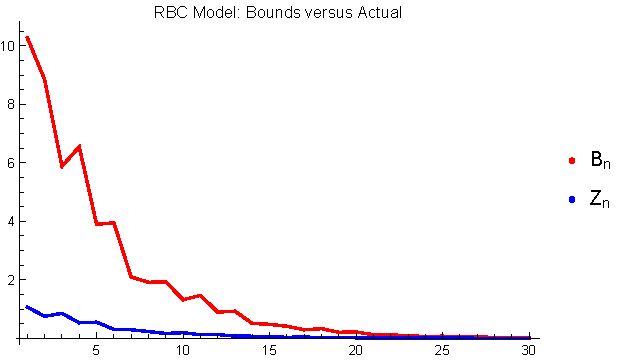
\includegraphics[width=1.7in]{simpArbBoundsVActual.pdf}  
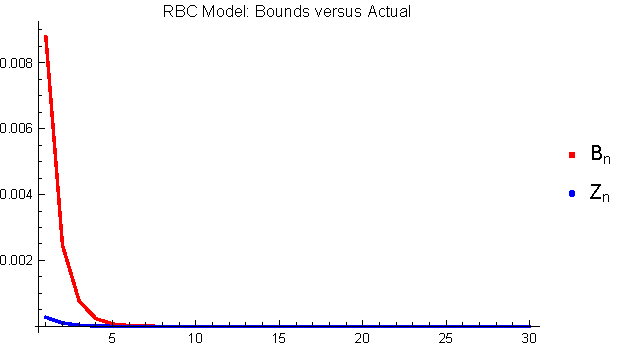
\includegraphics[width=1.7in]{simpBoundsVActual.pdf}  
  \caption{RBC Truncation Error Bound Versus Actual}
  \label{rbcTrunc}
\end{figure}
\end{frame}

\begin{frame}
  
  \begin{itemize}
  \item convenience of notation 
\begin{gather}
  h_i(x_{t-1},x_{t},x_{t+1},\epsilon_t)=h^{det}_{io}(x_{t-1},x_{t},\epsilon_t)+\\ \sum_{j=1}^{p_i} [h^{det}_{ij}(x_{t-1},x_{t},\epsilon_t)h^{nondet}_{ij}(x_{t+1})]=0
\intertext{For example, the Euler equations for the  neoclassical growth  model }
h_{10^{det}}(\cdot)=\frac{1}{c_t^\eta},\,\,
h_{11}^{det}()=\alpha \delta k_{t}^{\alpha-1} ,\,\,
h_{11}^{nondet}(\cdot)=E_t \left (\frac{\theta_{t+1}}{c_{t+1}^\eta} \right )\\
h_{20}^{det}(\cdot)=c_t + k_t-\theta_tk_{t-1}^\alpha,\,\,
h_{21}^{det}(\cdot)=0\\
h_{30}^{det}(\cdot)=\ln \theta_t -(\rho \ln \theta_{t-1} + \epsilon_t),\,\,
h_{31}^{det}(\cdot)=0
\end{gather}
  \end{itemize}

\end{frame}


\begin{frame}
  

\begin{itemize}
\item 
We now construct our linear reference model by increasing its dimension by one , $\linMod$, to accommodate 
 augmenting the RBC model with the equation
\begin{tcolorbox}[ams gather]
  \rcpC_t=\frac{\eta\theta_t}{c_t}
\end{tcolorbox}
substituting $\rcpC_{t+1}$ for $\frac{\theta_t}{c_{t+1}}$ in the first equation and 
 linearizing the RBC model about the ergodic mean
{\tiny
\begin{gather}
  \begin{bmatrix}
H_{-1}&H_{0}&H_{1} 
  \end{bmatrix}=\\
\vcenter{\hbox{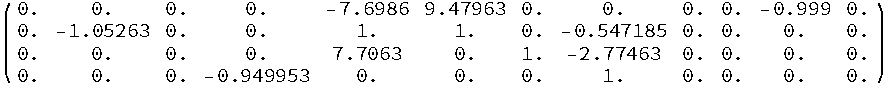
\includegraphics{RBCHmatSymb.pdf}}} \label{rbcLinSys}
\intertext{with}
\psi_\epsilon=
\begin{bmatrix}
  0\\0\\1\\0
\end{bmatrix}, \psi_z=I
\end{gather}%(\footnote{generated by AMAPaperCalcs.mth {RBCHmatSymb.pdf}})
}
\end{itemize}
\end{frame}

 \begin{frame}
  
 \begin{itemize}
\item 

These coefficients  produce a unique stable linear solution.
{\tiny
\begin{gather}
  B=
\vcenter{\hbox{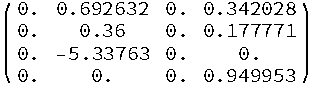
\includegraphics{RBCBmatSymb.pdf}}},\\
\phi=
\vcenter{\hbox{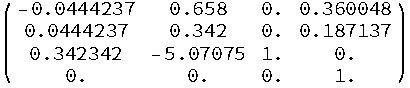
\includegraphics{RBCPhimatSymb.pdf}}}\\
F=
\vcenter{\hbox{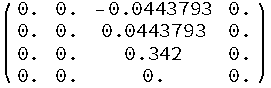
\includegraphics{RBCFmatSymb.pdf}}}\\
\psi_c=
\vcenter{\hbox{\includegraphics{RBCHSum.pdf}}}
\vcenter{\hbox{\includegraphics{RBCSS.pdf}}}=\vcenter{\hbox{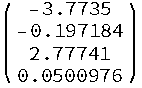
\includegraphics{RBCPsissSymb.pdf}}}
\end{gather}
}
 \end{itemize}
 \end{frame}

\section{A Model Error Bound}
\label{sec:bound}


\section{A New Solution Algorithm}
\label{sec:new-solut-algor}


\section{Conclusions}
\label{sec:conclusions}


\begin{frame}
  \frametitle{Next Steps}
\begin{itemize}
\item Support Vector Machine Regression (SVMR)
\item Large Model Implementation
\item Improve Error Bounds
\item Dynare Interface
\end{itemize}

\end{frame}



\bibliographystyle{plainnat}
\bibliography{anderson,files}

\end{document}
